For at beskrive integrationen og samspillet mellem en kørsel og
databasen vil der følge en beskrivelse af de vigtige kald mellem 
start.py og databasen. 
%intro til start.py
\subsection{Workflow}
%find på en bedre titel!
Start.py er distributør af arbejde til de andre dele af programkoden.
Diagram \ref{start_workflow} og pseudokode \ref{pseudo_workflow} giver et overblik over hvad der bliver
forklaret i resten af dette kapitel. 
\begin{figure}[h!]
	\begin{center}
		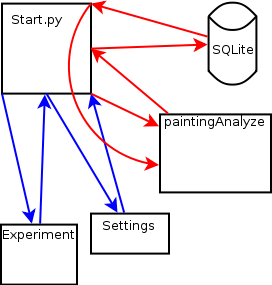
\includegraphics[scale=0.5]{afsnit/implementation/billeder/workflow_start_py.png}
	\end{center}
	\caption{De blå pile er ting, som sker en enkelt gang, mens de blå
	\label{start_workflow}
	bliver gentaget indtil der ikke er flere billeder at arbejde på}
\end{figure}
\begin{lstlisting}[caption={Pseudokode for
start},frame=tb,label={pseudo_workflow}
cuts = environment.generateCuts()
environment.setSettings(settings)
environment.setGlobalSettings(globalSettings)
db = Database(globalSettings)
run = m.createNewRun(settings)
paintings = m.Painting.select(m.Painting.q.form=="painting")
for painting in paintings:
	paintingContainer = Painting(painting)
	paintingContainer.setResults(paintingAnalyzer.analyze(paintingContainer,settings))
	m.saveResults(run.id,paintingContainer)
\end{lstlisting}
%Settings 
%konstruktion af databasen inklusiv downloading og crawling
%Loop
